\documentclass[a4paper,11pt]{article}

\usepackage{Sweave}

\usepackage{polyglossia}
    \setmainlanguage{english}

\usepackage{fontspec}
    \defaultfontfeatures{Mapping=tex-text}
    \setmainfont{Charis SIL}
    \frenchspacing



\title{Preliminary analysis}


\begin{document}
\input{analysis-concordance}
\maketitle


The following code loads the result file and the file containing the words of the task.

\begin{Schunk}
\begin{Sinput}
> results_raw <- read.csv("~/Documents/Projects/mathesis-is/analysis/results.csv")
> words <- read.csv("~/Documents/Projects/mathesis-is/task/task-src/words.csv")
\end{Sinput}
\end{Schunk}

Now we can merge the result and words files into one single data frame.

\begin{Schunk}
\begin{Sinput}
> results <- merge(results_raw, words, by.x = "word", by.y = "lex")
\end{Sinput}
\end{Schunk}

To check that the duration of each word token as spoken by the participants, we first need to split the data into two subsets: one with monosyllabic words and one with bisyllabic words.

\begin{Schunk}
\begin{Sinput}
> mono <- subset(results, syl_no == "mono")
> bi <- subset(results, syl_no == "bi")
\end{Sinput}
\end{Schunk}

We can now separately check the duration of monosyllabic and bisyllabic words.

\begin{Schunk}
\begin{Sinput}
> plot(
+     c(), c(),
+     xlim = c(0.1,0.9),
+     ylim = c(0,150),
+     xlab = "duration (s)", ylab = "frequency"
+ )
> hist(
+     mono$dur_word, add = TRUE, col = "darkgrey"
+ )
> hist(
+     bi$dur_word, add = TRUE, col = "lightgrey"
+ )
\end{Sinput}
\end{Schunk}
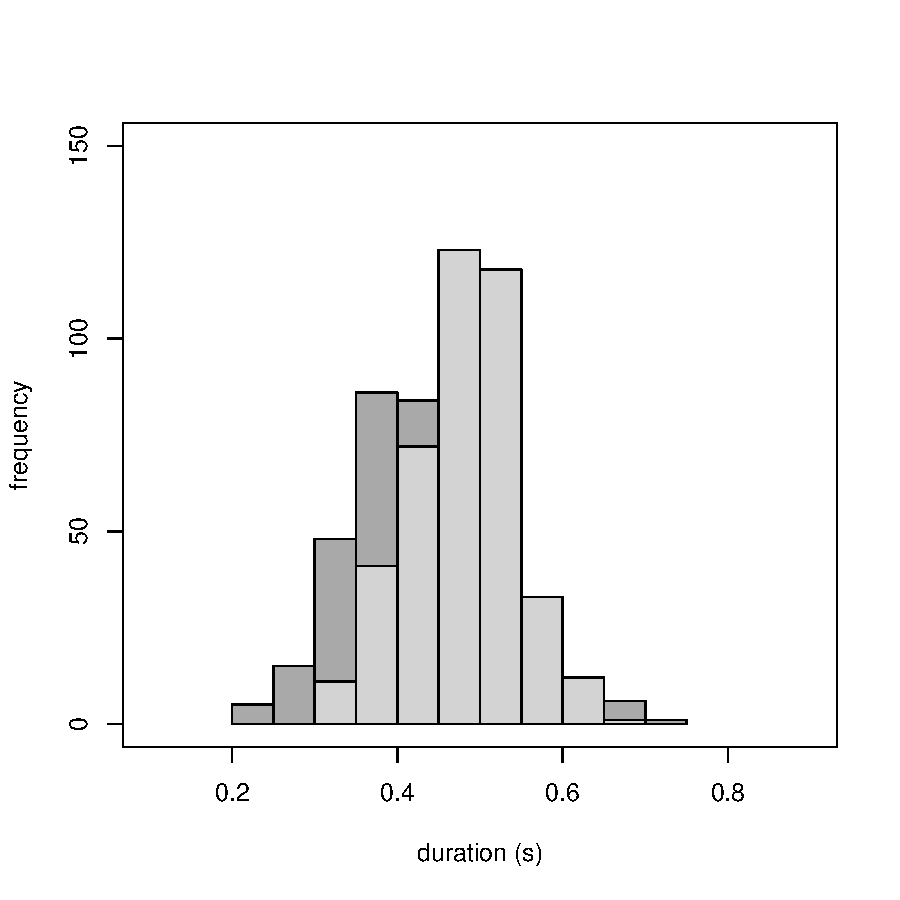
\includegraphics{analysis-004}

The mean length of monosyllabic words is 0.44s, while that of bisyllabic words is 0.48s.

Since I am looking at the duration of the normalised modal voicing of the vocalic gesture, we should first check if there is a significant difference in length of modal voicing between mono- and bisyllabic words.

\begin{Schunk}
\begin{Sinput}
> norm_abs_voic_mono_density <- density(mono$norm_abs_voic)
> norm_abs_voic_bi_density <- density(bi$norm_abs_voic)
> norm_abs_voic_density_x <- c(norm_abs_voic_mono_density$x, 
+                                   norm_abs_voic_bi_density$x)
> norm_abs_voic_density_y <- c(norm_abs_voic_mono_density$y, 
+                                   norm_abs_voic_bi_density$y)
> x.limits <- range(norm_abs_voic_density_x)
> y.limits <- range(norm_abs_voic_density_y)
> plot(
+ c(), c(),
+ xlim = x.limits,
+ ylim = y.limits,
+ xlab = "duration (s)", ylab = "density"
+ )
> lines(norm_abs_voic_mono_density, lw = 1, col = "blue")
> lines(norm_abs_voic_bi_density, lw = 1, col = "red")
\end{Sinput}
\end{Schunk}
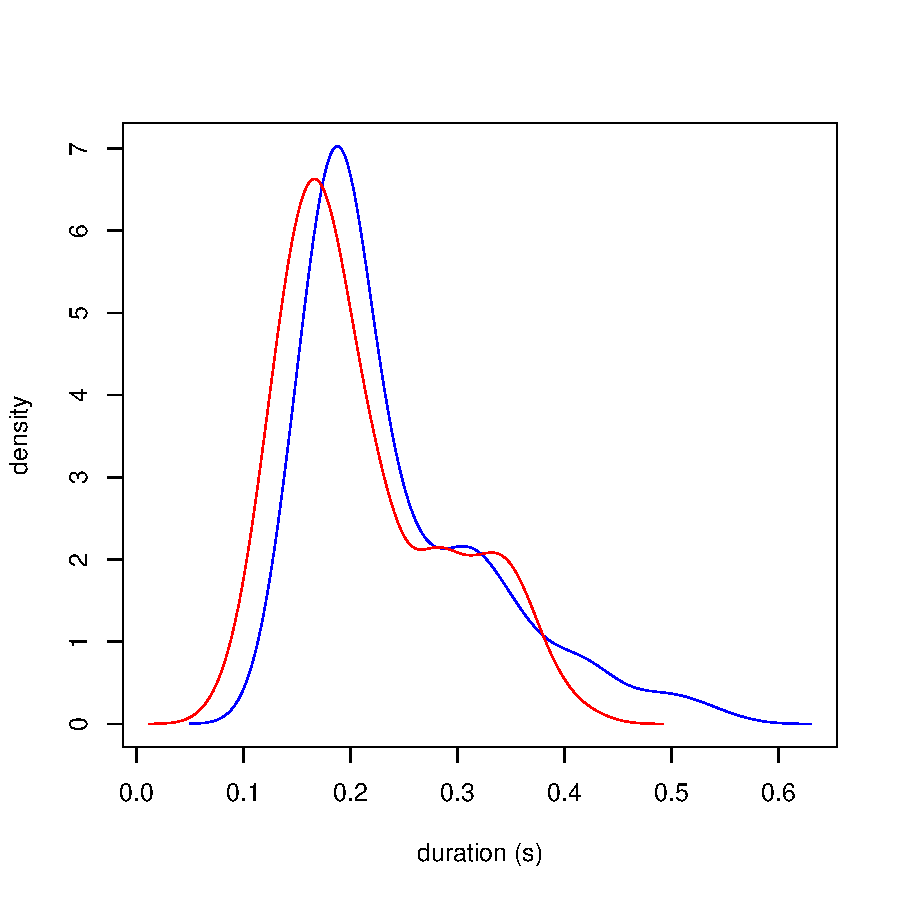
\includegraphics{analysis-005}

A two-sample unpaired \textit{t}-test shows that the length of modal voicing in words starting with an aspirated stop and ending in a stop is significantly longer in monosyllabic words than in bisyllabic words.
Subsequent tests will be performed for monosyllabic and bisyllabic words separately.

\begin{Schunk}
\begin{Sinput}
> mono_stop <- subset(mono, manner == "stop")
> bi_stop <- subset(bi, manner == "stop")
> t.test(mono_stop$norm_abs_voic, bi_stop$norm_abs_voic)
\end{Sinput}
\begin{Soutput}
	Welch Two Sample t-test

data:  mono_stop$norm_abs_voic and bi_stop$norm_abs_voic
t = 6.341, df = 473.48, p-value = 5.333e-10
alternative hypothesis: true difference in means is not equal to 0
95 percent confidence interval:
 0.0345702 0.0656167
sample estimates:
mean of x mean of y 
0.2611856 0.2110922 
\end{Soutput}
\end{Schunk}

\section{Monosyllabic words}

\subsection{Stops}

We can now have a look at monosyllabic words, starting from CVCC words (ending in a geminate stop).
These words start with either an aspirated, a non-aspirated or a sonorant consonant.
Words starting with a voiced fricative are treated separately?
Maybe I should not treat them separately.

\begin{Schunk}
\begin{Sinput}
> mono_stop_asp <- mono_stop$norm_abs_voic[mono_stop$asp == "yes"]
> mono_stop_nasp <- mono_stop$norm_abs_voic[mono_stop$asp == "no"]
> norm_abs_voic_asp_density <- density(mono_stop_asp)
> norm_abs_voic_nasp_density <- density(mono_stop_nasp)
> norm_abs_voic_density_x <- c(norm_abs_voic_asp_density$x, 
+                                   norm_abs_voic_nasp_density$x)
> norm_abs_voic_density_y <- c(norm_abs_voic_asp_density$y, 
+                                   norm_abs_voic_nasp_density$y)
> x.limits <- range(norm_abs_voic_density_x)
> y.limits <- range(norm_abs_voic_density_y)
> plot(
+ c(), c(),
+ xlim = x.limits,
+ ylim = y.limits,
+ xlab = "duration (s)", ylab = "density"
+ )
> lines(norm_abs_voic_asp_density, lw = 1, col = "blue")
> lines(norm_abs_voic_nasp_density, lw = 1, col = "red")
\end{Sinput}
\end{Schunk}
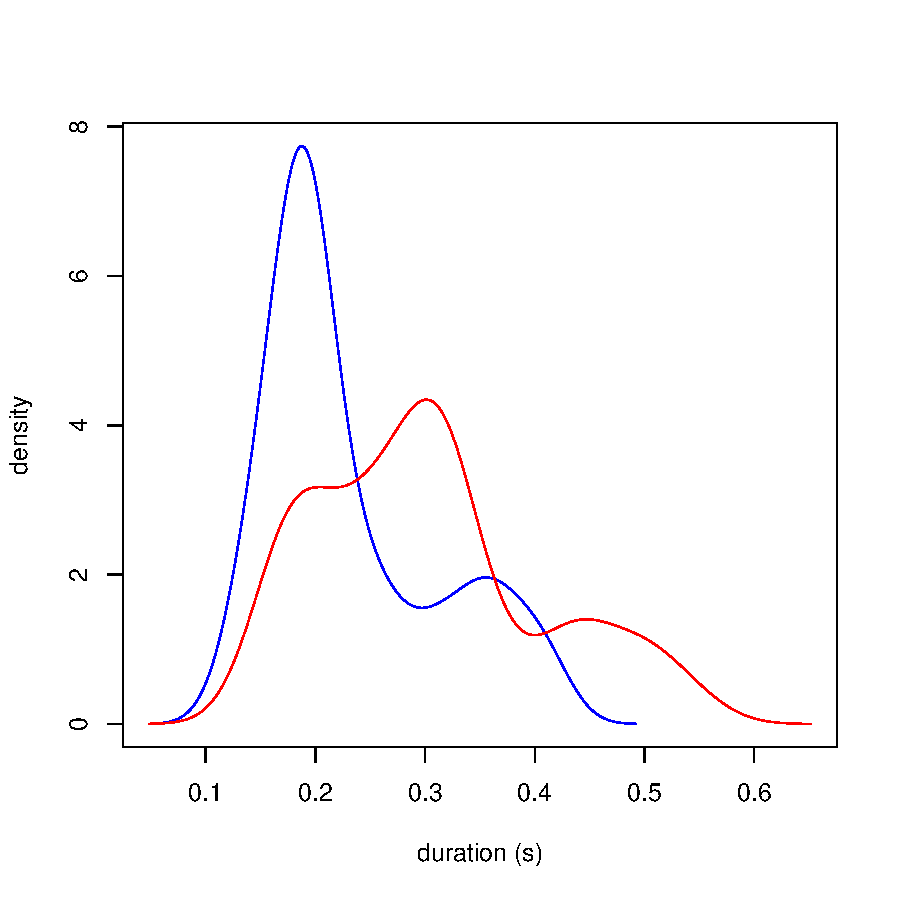
\includegraphics{analysis-007}

\begin{Schunk}
\begin{Sinput}
> shapiro.test(mono_stop_asp)
\end{Sinput}
\begin{Soutput}
	Shapiro-Wilk normality test

data:  mono_stop_asp
W = 0.87625, p-value = 1.213e-10
\end{Soutput}
\begin{Sinput}
> shapiro.test(mono_stop_nasp)
\end{Sinput}
\begin{Soutput}
	Shapiro-Wilk normality test

data:  mono_stop_nasp
W = 0.94458, p-value = 6.258e-05
\end{Soutput}
\end{Schunk}

Since the distributions of the duration of modal voicing in the two conditions (pre-aspirated and non-aspirated) are significantly different from the normal distribution, we should perform a Wilcoxon test.
According to the test, the mean duration of modal voicing in words ending with a pre-aspirated stop is significantly shorter (0.23 seconds) than in words ending with a non-aspirated stop (0.3 seconds).

\begin{Schunk}
\begin{Sinput}
> boxplot(norm_abs_voic ~ asp,
+         data = mono_stop,
+         names = c("non-asp", "asp"),
+         ylab = "duration (s)",
+         main = "Duration (in seconds) of modal voicing in CVCC words"
+         )
> wilcox.test(norm_abs_voic ~ asp, data = mono_stop)
\end{Sinput}
\begin{Soutput}
	Wilcoxon rank sum test with continuity correction

data:  norm_abs_voic by asp
W = 14935, p-value = 2.642e-09
alternative hypothesis: true location shift is not equal to 0
\end{Soutput}
\end{Schunk}
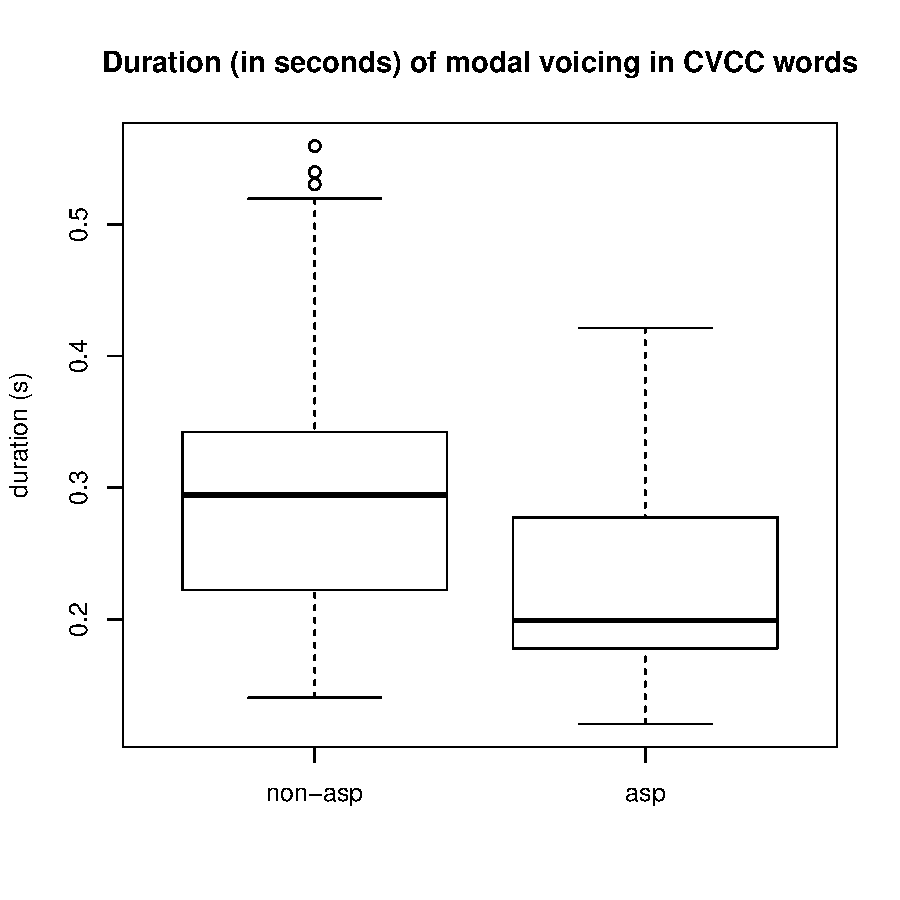
\includegraphics{analysis-009}

\subsection{Nasals}

\begin{Schunk}
\begin{Sinput}
> mono_nas <- subset(mono, manner == "nasal")
\end{Sinput}
\end{Schunk}

\begin{Schunk}
\begin{Sinput}
> mono_nas_asp <- mono_nas$norm_abs_voic[mono_nas$asp == "yes"]
> mono_nas_nasp <- mono_nas$norm_abs_voic[mono_nas$asp == "no"]
> norm_abs_voic_asp_density <- density(mono_nas_asp)
> norm_abs_voic_nasp_density <- density(mono_nas_nasp)
> norm_abs_voic_density_x <- c(norm_abs_voic_asp_density$x, 
+                                   norm_abs_voic_nasp_density$x)
> norm_abs_voic_density_y <- c(norm_abs_voic_asp_density$y, 
+                                   norm_abs_voic_nasp_density$y)
> x.limits <- range(norm_abs_voic_density_x)
> y.limits <- range(norm_abs_voic_density_y)
> plot(
+ c(), c(),
+ xlim = x.limits,
+ ylim = y.limits,
+ xlab = "duration (s)", ylab = "density"
+ )
> lines(norm_abs_voic_asp_density, lw = 1, col = "blue")
> lines(norm_abs_voic_nasp_density, lw = 1, col = "red")
\end{Sinput}
\end{Schunk}
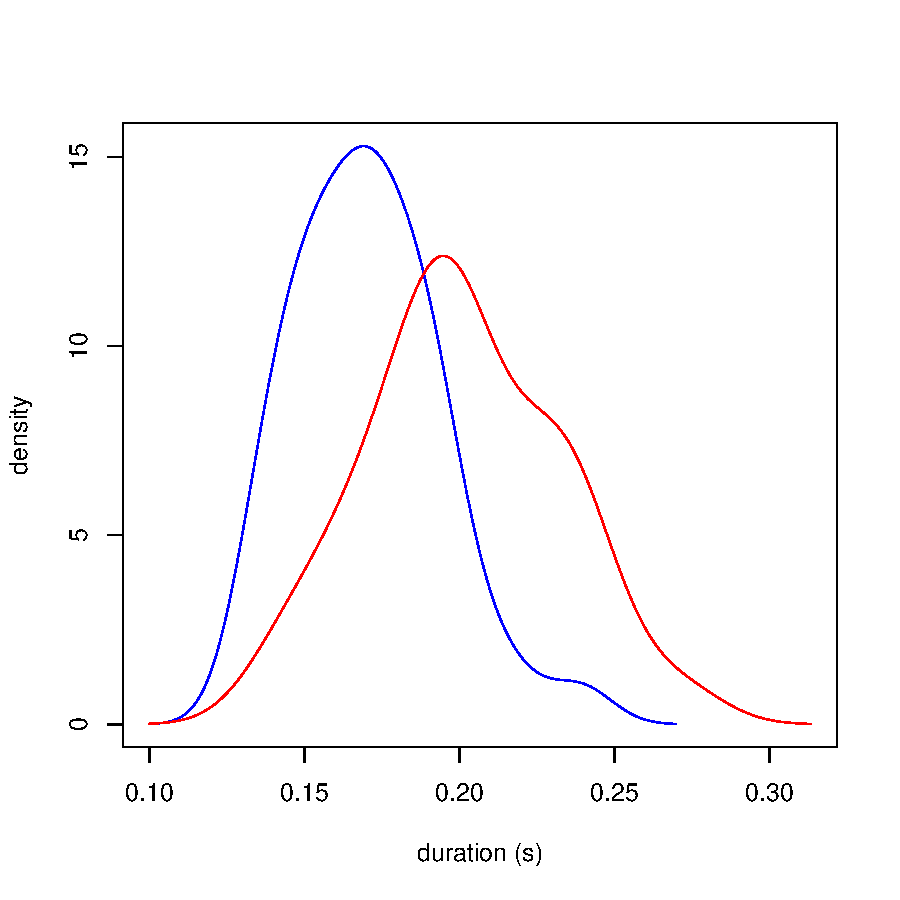
\includegraphics{analysis-011}

\begin{Schunk}
\begin{Sinput}
> boxplot(norm_abs_voic ~ asp,
+         data = mono_nas,
+         names = c("non-asp", "asp"),
+         ylab = "duration (s)",
+         main = "Duration (in seconds) of modal voicing in CVNC words"
+         )
\end{Sinput}
\end{Schunk}
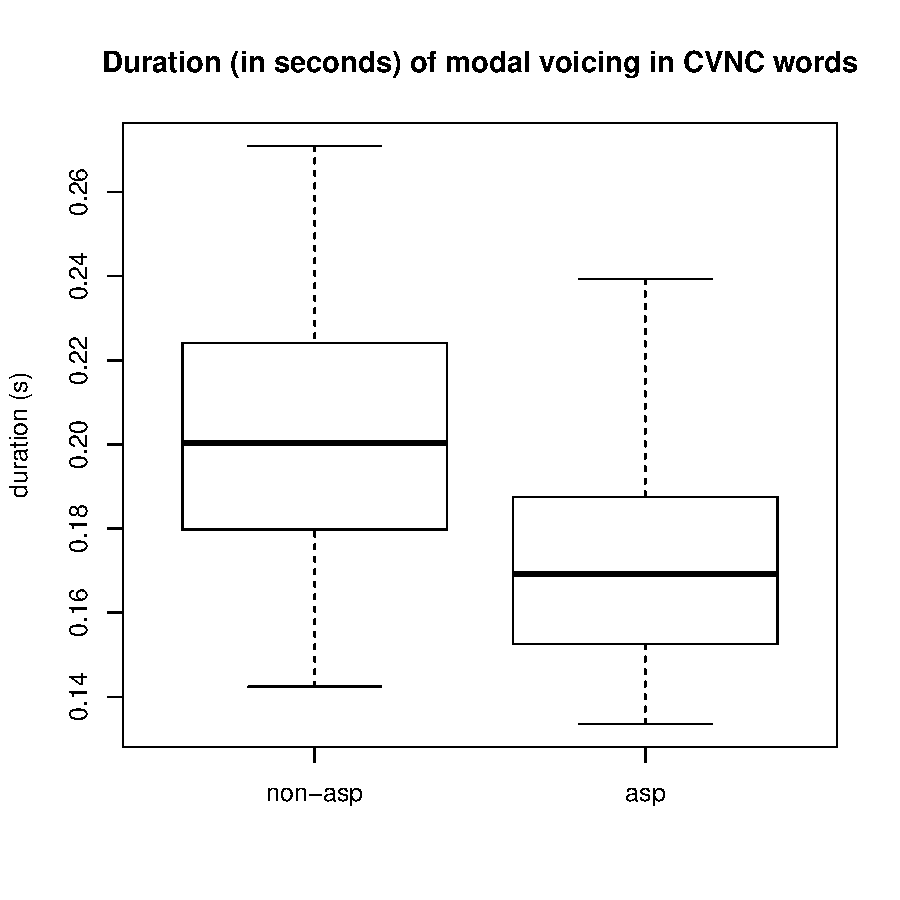
\includegraphics{analysis-012}

\begin{Schunk}
\begin{Sinput}
> shapiro.test(mono_nas_asp)
\end{Sinput}
\begin{Soutput}
	Shapiro-Wilk normality test

data:  mono_nas_asp
W = 0.96651, p-value = 0.2776
\end{Soutput}
\begin{Sinput}
> shapiro.test(mono_nas_nasp)
\end{Sinput}
\begin{Soutput}
	Shapiro-Wilk normality test

data:  mono_nas_nasp
W = 0.98409, p-value = 0.9277
\end{Soutput}
\begin{Sinput}
> t.test(norm_abs_voic ~ asp, data = mono_nas)
\end{Sinput}
\begin{Soutput}
	Welch Two Sample t-test

data:  norm_abs_voic by asp
t = 4.4883, df = 50.272, p-value = 4.202e-05
alternative hypothesis: true difference in means is not equal to 0
95 percent confidence interval:
 0.01693745 0.04436910
sample estimates:
 mean in group no mean in group yes 
        0.2010632         0.1704099 
\end{Soutput}
\end{Schunk}

According to a two-sample \textit{t}-test, the duration of modal voicing in words ending with an N̥C cluster (0.17 seconds) is shorter than in words ending with an NC cluster (0.2 seconds).

\subsection{Laterals}

\begin{Schunk}
\begin{Sinput}
> mono_lat <- subset(mono, manner == "lateral")
\end{Sinput}
\end{Schunk}

\begin{Schunk}
\begin{Sinput}
> mono_lat_asp <- mono_lat$norm_abs_voic[mono_lat$asp == "yes"]
> mono_lat_nasp <- mono_lat$norm_abs_voic[mono_lat$asp == "no"]
> norm_abs_voic_asp_density <- density(mono_lat_asp)
> norm_abs_voic_nasp_density <- density(mono_lat_nasp)
> norm_abs_voic_density_x <- c(norm_abs_voic_asp_density$x, 
+                                   norm_abs_voic_nasp_density$x)
> norm_abs_voic_density_y <- c(norm_abs_voic_asp_density$y, 
+                                   norm_abs_voic_nasp_density$y)
> x.limits <- range(norm_abs_voic_density_x)
> y.limits <- range(norm_abs_voic_density_y)
> plot(
+ c(), c(),
+ xlim = x.limits,
+ ylim = y.limits,
+ xlab = "duration (s)", ylab = "density"
+ )
> lines(norm_abs_voic_asp_density, lw = 1, col = "blue")
> lines(norm_abs_voic_nasp_density, lw = 1, col = "red")
\end{Sinput}
\end{Schunk}
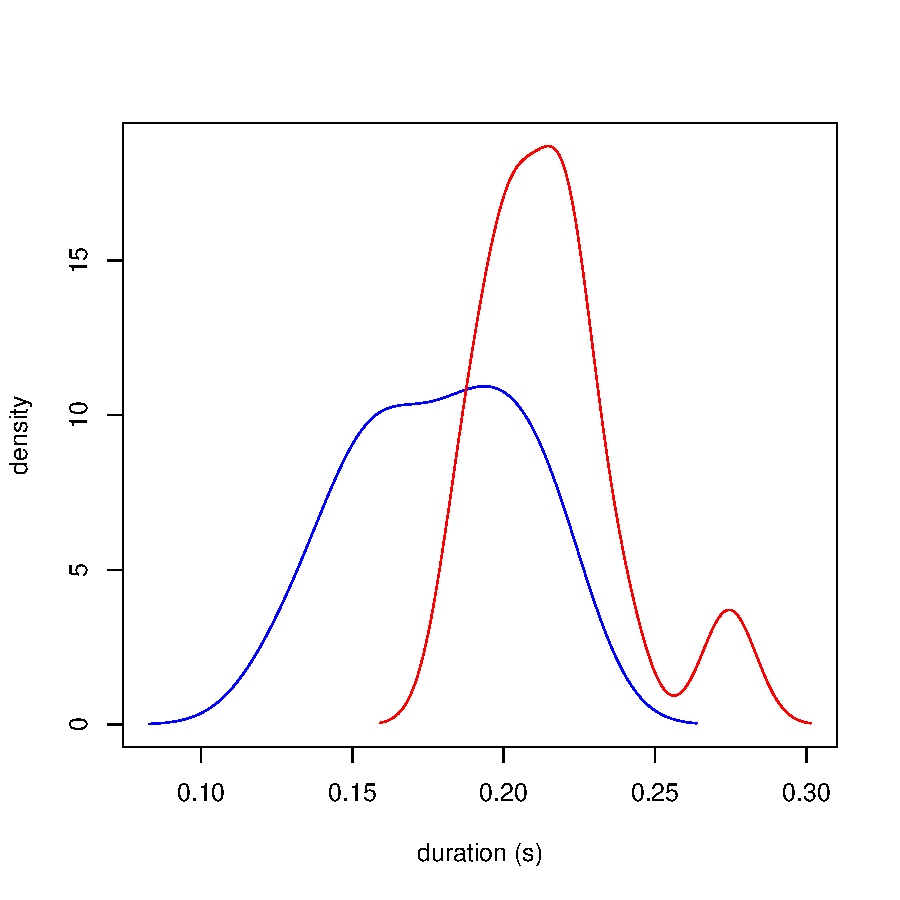
\includegraphics{analysis-015}

\begin{Schunk}
\begin{Sinput}
> boxplot(norm_abs_voic ~ asp,
+         data = mono_lat,
+         names = c("non-asp", "asp"),
+         ylab = "duration (s)",
+         main = "Duration (in seconds) of modal voicing in CVLC words"
+         )
\end{Sinput}
\end{Schunk}
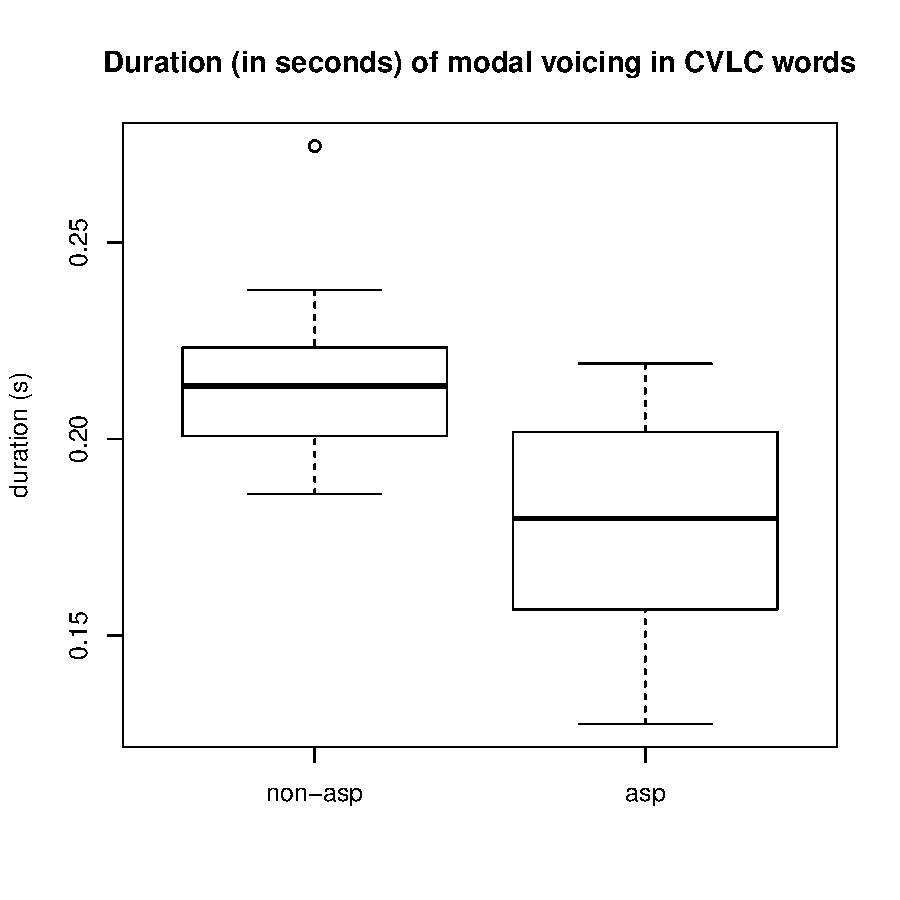
\includegraphics{analysis-016}

\begin{Schunk}
\begin{Sinput}
> shapiro.test(mono_lat_asp)
\end{Sinput}
\begin{Soutput}
	Shapiro-Wilk normality test

data:  mono_lat_asp
W = 0.96233, p-value = 0.7329
\end{Soutput}
\begin{Sinput}
> shapiro.test(mono_lat_nasp)
\end{Sinput}
\begin{Soutput}
	Shapiro-Wilk normality test

data:  mono_lat_nasp
W = 0.8995, p-value = 0.1563
\end{Soutput}
\begin{Sinput}
> t.test(norm_abs_voic ~ asp, data = mono_lat)
\end{Sinput}
\begin{Soutput}
	Welch Two Sample t-test

data:  norm_abs_voic by asp
t = 3.6588, df = 24.907, p-value = 0.001188
alternative hypothesis: true difference in means is not equal to 0
95 percent confidence interval:
 0.01609712 0.05757378
sample estimates:
 mean in group no mean in group yes 
        0.2154738         0.1786384 
\end{Soutput}
\end{Schunk}

It is good to check whether the duration of monosyllabic words is affected by the presence vs. absence of preaspiration.

\begin{Schunk}
\begin{Sinput}
> boxplot(dur_word ~ asp, data = mono)
> shapiro.test(mono$dur_word[mono$asp == "yes"])
\end{Sinput}
\begin{Soutput}
	Shapiro-Wilk normality test

data:  mono$dur_word[mono$asp == "yes"]
W = 0.98839, p-value = 0.06551
\end{Soutput}
\begin{Sinput}
> shapiro.test(mono$dur_word[mono$asp == "no"])
\end{Sinput}
\begin{Soutput}
	Shapiro-Wilk normality test

data:  mono$dur_word[mono$asp == "no"]
W = 0.98788, p-value = 0.1235
\end{Soutput}
\end{Schunk}
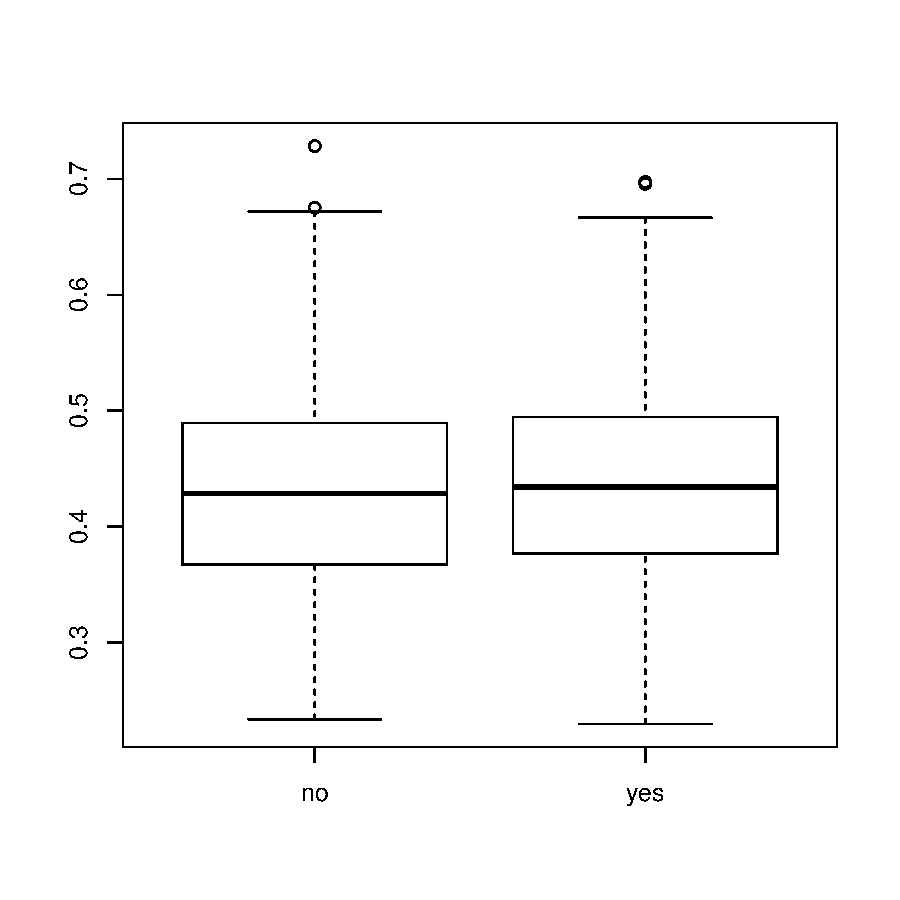
\includegraphics{analysis-018}

\begin{Schunk}
\begin{Sinput}
> t.test(dur_word ~ asp, data = mono)
\end{Sinput}
\begin{Soutput}
	Welch Two Sample t-test

data:  dur_word by asp
t = -0.33834, df = 358.51, p-value = 0.7353
alternative hypothesis: true difference in means is not equal to 0
95 percent confidence interval:
 -0.02081099  0.01470130
sample estimates:
 mean in group no mean in group yes 
        0.4336616         0.4367164 
\end{Soutput}
\end{Schunk}

According to a \textit{t}-test, the duration of monosyllabic words is not affected by the presence vs. absence of preaspiration.
Thus, difference in the mean duration of modal voicing can't be attributed to differences in word duration. 

\section{Bisyllabic words}

\subsection{Stops}

\begin{Schunk}
\begin{Sinput}
> bi_stop_asp <- bi_stop$norm_abs_voic[bi_stop$asp == "yes"]
> bi_stop_nasp <- bi_stop$norm_abs_voic[bi_stop$asp == "no"]
> norm_abs_voic_asp_density <- density(bi_stop_asp)
> norm_abs_voic_nasp_density <- density(bi_stop_nasp)
> norm_abs_voic_density_x <- c(norm_abs_voic_asp_density$x, 
+                                   norm_abs_voic_nasp_density$x)
> norm_abs_voic_density_y <- c(norm_abs_voic_asp_density$y, 
+                                   norm_abs_voic_nasp_density$y)
> x.limits <- range(norm_abs_voic_density_x)
> y.limits <- range(norm_abs_voic_density_y)
> plot(
+ c(), c(),
+ xlim = x.limits,
+ ylim = y.limits,
+ xlab = "duration (s)", ylab = "density"
+ )
> lines(norm_abs_voic_asp_density, lw = 1, col = "blue")
> lines(norm_abs_voic_nasp_density, lw = 1, col = "red")
\end{Sinput}
\end{Schunk}
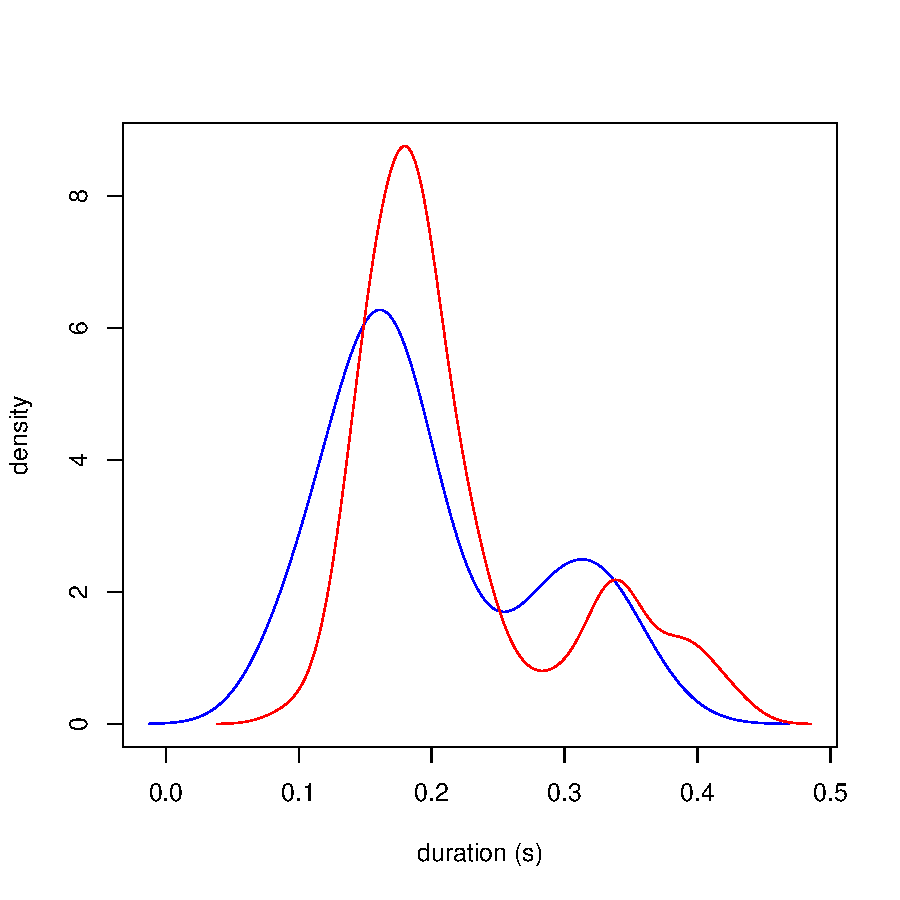
\includegraphics{analysis-020}

\begin{Schunk}
\begin{Sinput}
> shapiro.test(bi_stop_asp)
\end{Sinput}
\begin{Soutput}
	Shapiro-Wilk normality test

data:  bi_stop_asp
W = 0.91525, p-value = 3.106e-05
\end{Soutput}
\begin{Sinput}
> shapiro.test(bi_stop_nasp)
\end{Sinput}
\begin{Soutput}
	Shapiro-Wilk normality test

data:  bi_stop_nasp
W = 0.8522, p-value = 3.024e-09
\end{Soutput}
\end{Schunk}

\begin{Schunk}
\begin{Sinput}
> boxplot(norm_abs_voic ~ asp,
+         data = bi_stop,
+         names = c("non-asp", "asp"),
+         ylab = "duration (s)",
+         main = "Duration (in seconds) of modal voicing in CVCCV words"
+         )
> wilcox.test(norm_abs_voic ~ asp, data = mono_stop)
\end{Sinput}
\begin{Soutput}
	Wilcoxon rank sum test with continuity correction

data:  norm_abs_voic by asp
W = 14935, p-value = 2.642e-09
alternative hypothesis: true location shift is not equal to 0
\end{Soutput}
\end{Schunk}
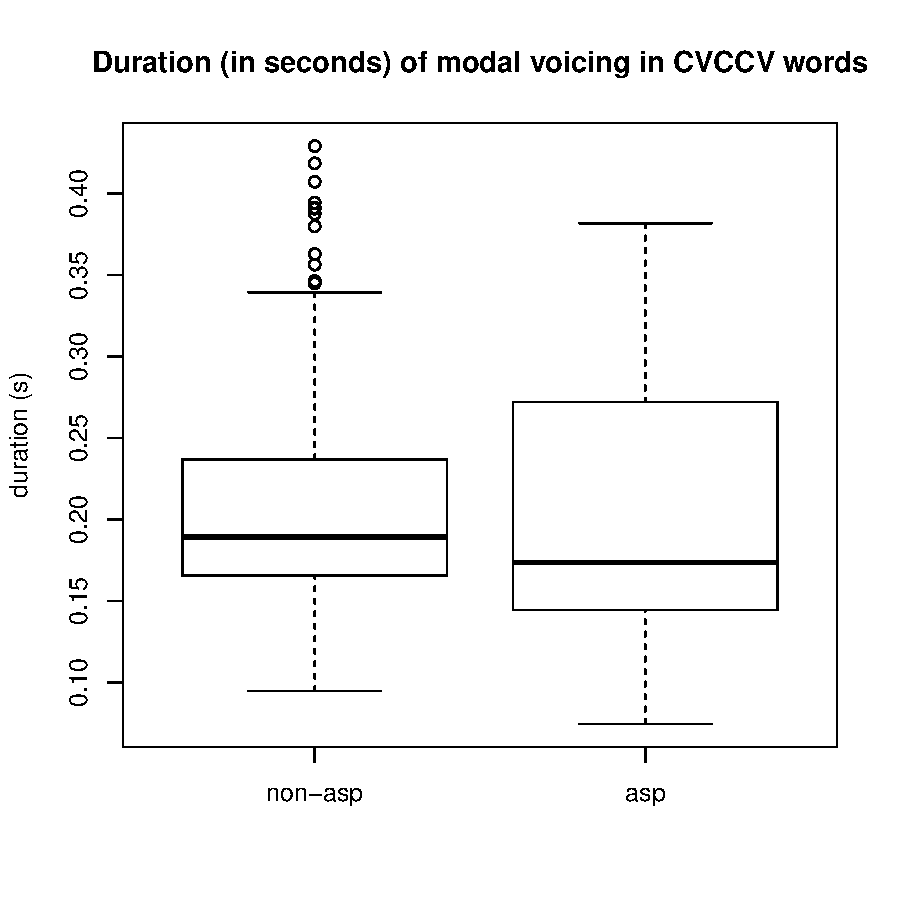
\includegraphics{analysis-022}

\subsection{Nasals}

\begin{Schunk}
\begin{Sinput}
> bi_nas <- subset(bi, manner == "nasal")
\end{Sinput}
\end{Schunk}

\begin{Schunk}
\begin{Sinput}
> bi_nas_asp <- bi_nas$norm_abs_voic[bi_nas$asp == "yes"]
> bi_nas_nasp <- bi_nas$norm_abs_voic[bi_nas$asp == "no"]
> norm_abs_voic_asp_density <- density(bi_nas_asp)
> norm_abs_voic_nasp_density <- density(bi_nas_nasp)
> norm_abs_voic_density_x <- c(norm_abs_voic_asp_density$x, 
+                                   norm_abs_voic_nasp_density$x)
> norm_abs_voic_density_y <- c(norm_abs_voic_asp_density$y, 
+                                   norm_abs_voic_nasp_density$y)
> x.limits <- range(norm_abs_voic_density_x)
> y.limits <- range(norm_abs_voic_density_y)
> plot(
+ c(), c(),
+ xlim = x.limits,
+ ylim = y.limits,
+ xlab = "duration (s)", ylab = "density"
+ )
> lines(norm_abs_voic_asp_density, lw = 1, col = "blue")
> lines(norm_abs_voic_nasp_density, lw = 1, col = "red")
\end{Sinput}
\end{Schunk}
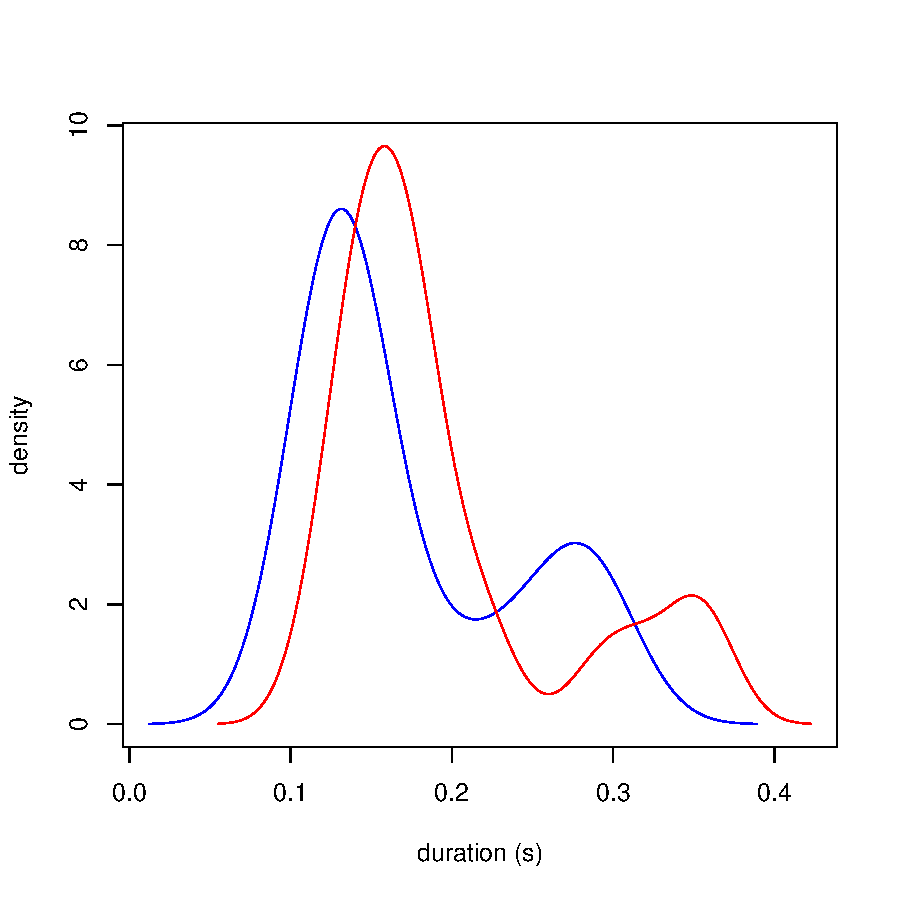
\includegraphics{analysis-024}

\begin{Schunk}
\begin{Sinput}
> boxplot(norm_abs_voic ~ asp,
+         data = bi_nas,
+         names = c("non-asp", "asp"),
+         ylab = "duration (s)",
+         main = "Duration (in seconds) of modal voicing in CVNCV words"
+         )
\end{Sinput}
\end{Schunk}
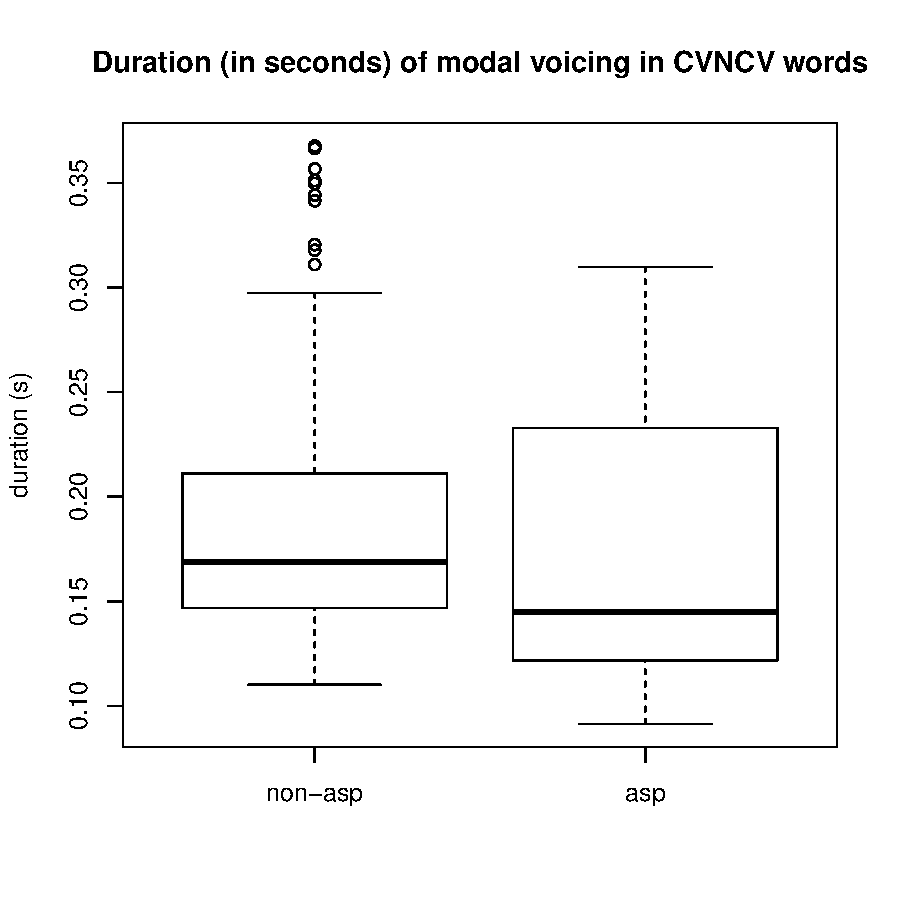
\includegraphics{analysis-025}

\begin{Schunk}
\begin{Sinput}
> shapiro.test(bi_nas_asp)
\end{Sinput}
\begin{Soutput}
	Shapiro-Wilk normality test

data:  bi_nas_asp
W = 0.82516, p-value = 1.012e-06
\end{Soutput}
\begin{Sinput}
> shapiro.test(bi_nas_nasp)
\end{Sinput}
\begin{Soutput}
	Shapiro-Wilk normality test

data:  bi_nas_nasp
W = 0.81301, p-value = 7.472e-08
\end{Soutput}
\begin{Sinput}
> wilcox.test(norm_abs_voic ~ asp, data = bi_nas)
\end{Sinput}
\begin{Soutput}
	Wilcoxon rank sum test with continuity correction

data:  norm_abs_voic by asp
W = 2515, p-value = 0.004268
alternative hypothesis: true location shift is not equal to 0
\end{Soutput}
\end{Schunk}

\subsection{Laterals}

\begin{Schunk}
\begin{Sinput}
> bi_lat <- subset(bi, manner == "lateral")
\end{Sinput}
\end{Schunk}

\begin{Schunk}
\begin{Sinput}
> bi_lat_asp <- bi_lat$norm_abs_voic[bi_lat$asp == "yes"]
> bi_lat_nasp <- bi_lat$norm_abs_voic[bi_lat$asp == "no"]
> norm_abs_voic_asp_density <- density(bi_lat_asp)
> norm_abs_voic_nasp_density <- density(bi_lat_nasp)
> norm_abs_voic_density_x <- c(norm_abs_voic_asp_density$x, 
+                                   norm_abs_voic_nasp_density$x)
> norm_abs_voic_density_y <- c(norm_abs_voic_asp_density$y, 
+                                   norm_abs_voic_nasp_density$y)
> x.limits <- range(norm_abs_voic_density_x)
> y.limits <- range(norm_abs_voic_density_y)
> plot(
+ c(), c(),
+ xlim = x.limits,
+ ylim = y.limits,
+ xlab = "duration (s)", ylab = "density"
+ )
> lines(norm_abs_voic_asp_density, lw = 1, col = "blue")
> lines(norm_abs_voic_nasp_density, lw = 1, col = "red")
\end{Sinput}
\end{Schunk}
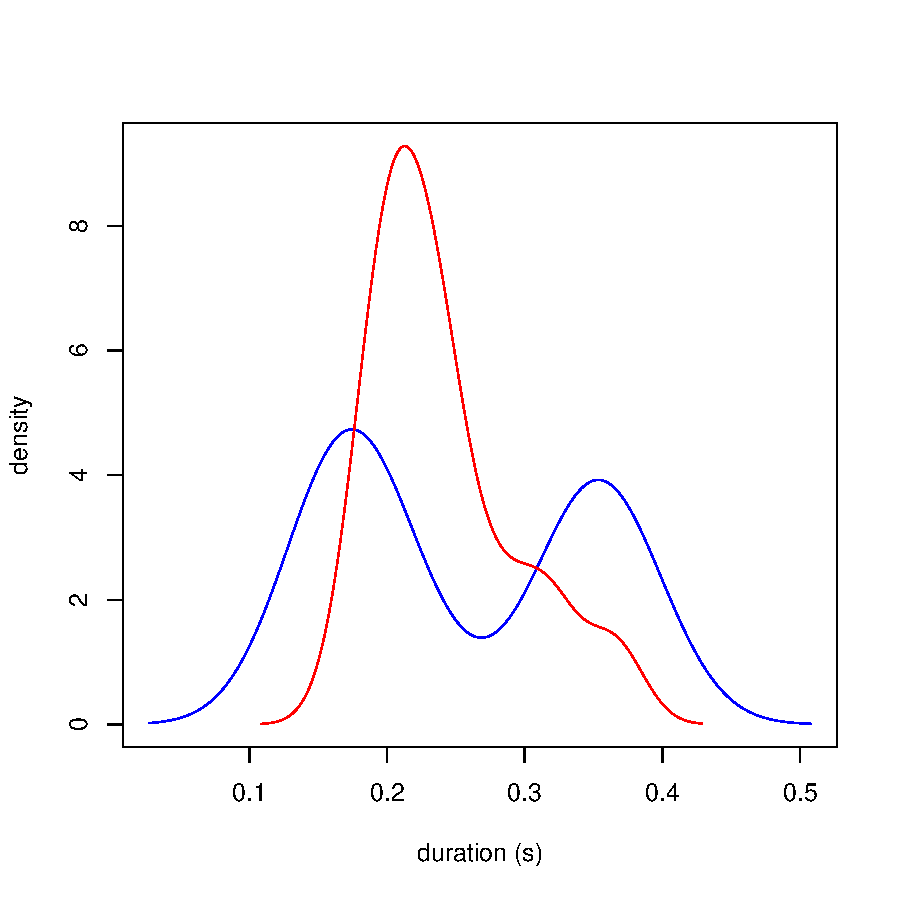
\includegraphics{analysis-028}

\begin{Schunk}
\begin{Sinput}
> boxplot(norm_abs_voic ~ asp,
+         data = bi_lat,
+         names = c("non-asp", "asp"),
+         ylab = "duration (s)",
+         main = "Duration (in seconds) of modal voicing in CVLCV words"
+         )
\end{Sinput}
\end{Schunk}
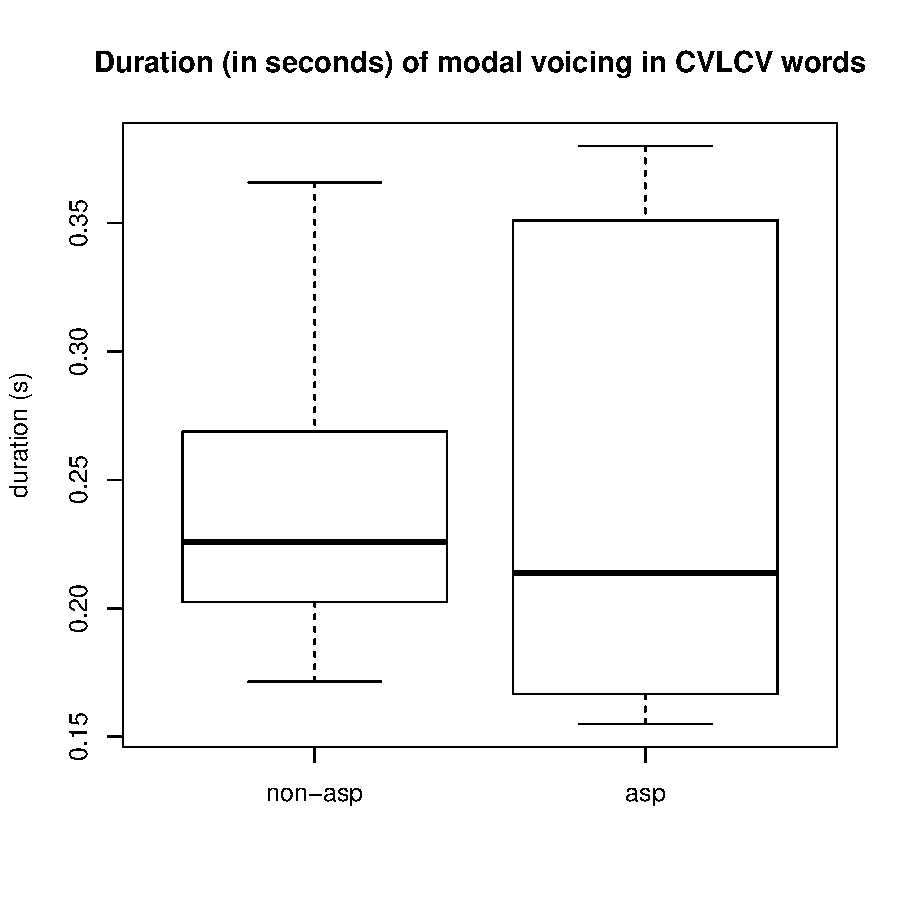
\includegraphics{analysis-029}

\begin{Schunk}
\begin{Sinput}
> shapiro.test(bi_lat_asp)
\end{Sinput}
\begin{Soutput}
	Shapiro-Wilk normality test

data:  bi_lat_asp
W = 0.78115, p-value = 6.565e-05
\end{Soutput}
\begin{Sinput}
> shapiro.test(bi_lat_nasp)
\end{Sinput}
\begin{Soutput}
	Shapiro-Wilk normality test

data:  bi_lat_nasp
W = 0.88907, p-value = 0.004586
\end{Soutput}
\begin{Sinput}
> wilcox.test(norm_abs_voic ~ asp, data = bi_lat)
\end{Sinput}
\begin{Soutput}
	Wilcoxon rank sum test

data:  norm_abs_voic by asp
W = 433, p-value = 0.6627
alternative hypothesis: true location shift is not equal to 0
\end{Soutput}
\end{Schunk}

\subsection{Rhotics}

\begin{Schunk}
\begin{Sinput}
> bi_rho <- subset(bi, manner == "rhotic")
\end{Sinput}
\end{Schunk}

\begin{Schunk}
\begin{Sinput}
> bi_rho_asp <- bi_rho$norm_abs_voic[bi_rho$asp == "yes"]
> bi_rho_nasp <- bi_rho$norm_abs_voic[bi_rho$asp == "no"]
> norm_abs_voic_asp_density <- density(bi_rho_asp)
> norm_abs_voic_nasp_density <- density(bi_rho_nasp)
> norm_abs_voic_density_x <- c(norm_abs_voic_asp_density$x, 
+                                   norm_abs_voic_nasp_density$x)
> norm_abs_voic_density_y <- c(norm_abs_voic_asp_density$y, 
+                                   norm_abs_voic_nasp_density$y)
> x.limits <- range(norm_abs_voic_density_x)
> y.limits <- range(norm_abs_voic_density_y)
> plot(
+ c(), c(),
+ xlim = x.limits,
+ ylim = y.limits,
+ xlab = "duration (s)", ylab = "density"
+ )
> lines(norm_abs_voic_asp_density, lw = 1, col = "blue")
> lines(norm_abs_voic_nasp_density, lw = 1, col = "red")
\end{Sinput}
\end{Schunk}
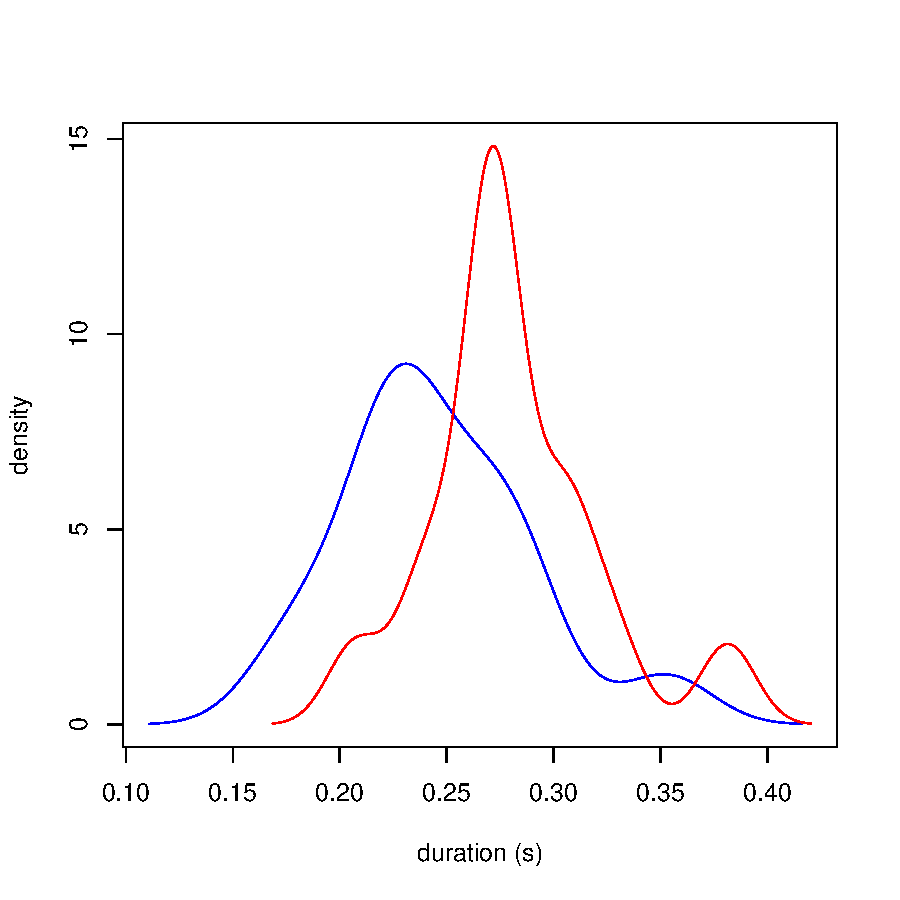
\includegraphics{analysis-032}

\begin{Schunk}
\begin{Sinput}
> boxplot(norm_abs_voic ~ asp,
+         data = bi_rho,
+         names = c("non-asp", "asp"),
+         ylab = "duration (s)",
+         main = "Duration (in seconds) of modal voicing in CVRCV words"
+         )
\end{Sinput}
\end{Schunk}
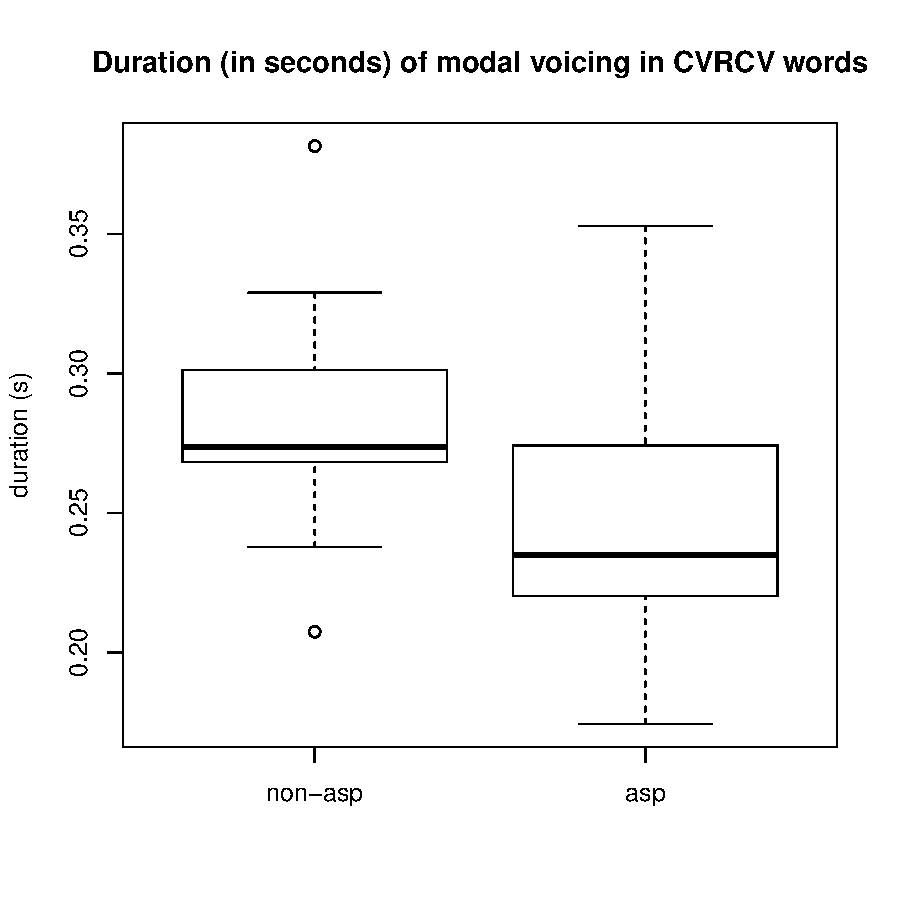
\includegraphics{analysis-033}

\begin{Schunk}
\begin{Sinput}
> shapiro.test(bi_rho_asp)
\end{Sinput}
\begin{Soutput}
	Shapiro-Wilk normality test

data:  bi_rho_asp
W = 0.9483, p-value = 0.4982
\end{Soutput}
\begin{Sinput}
> shapiro.test(bi_rho_nasp)
\end{Sinput}
\begin{Soutput}
	Shapiro-Wilk normality test

data:  bi_rho_nasp
W = 0.93249, p-value = 0.2972
\end{Soutput}
\begin{Sinput}
> t.test(norm_abs_voic ~ asp, data = bi_rho)
\end{Sinput}
\begin{Soutput}
	Welch Two Sample t-test

data:  norm_abs_voic by asp
t = 2.2691, df = 27.797, p-value = 0.03122
alternative hypothesis: true difference in means is not equal to 0
95 percent confidence interval:
 0.003433211 0.067391206
sample estimates:
 mean in group no mean in group yes 
        0.2808275         0.2454153 
\end{Soutput}
\end{Schunk}

As with monosyllabic words, we should check if the duration of bisyllabic words is affected by the presence vs. absence of preaspiration.

\begin{Schunk}
\begin{Sinput}
> boxplot(dur_word ~ asp, data = bi)
> shapiro.test(bi$dur_word[bi$asp == "yes"])
\end{Sinput}
\begin{Soutput}
	Shapiro-Wilk normality test

data:  bi$dur_word[bi$asp == "yes"]
W = 0.99244, p-value = 0.4518
\end{Soutput}
\begin{Sinput}
> shapiro.test(bi$dur_word[bi$asp == "no"])
\end{Sinput}
\begin{Soutput}
	Shapiro-Wilk normality test

data:  bi$dur_word[bi$asp == "no"]
W = 0.98318, p-value = 0.008744
\end{Soutput}
\end{Schunk}
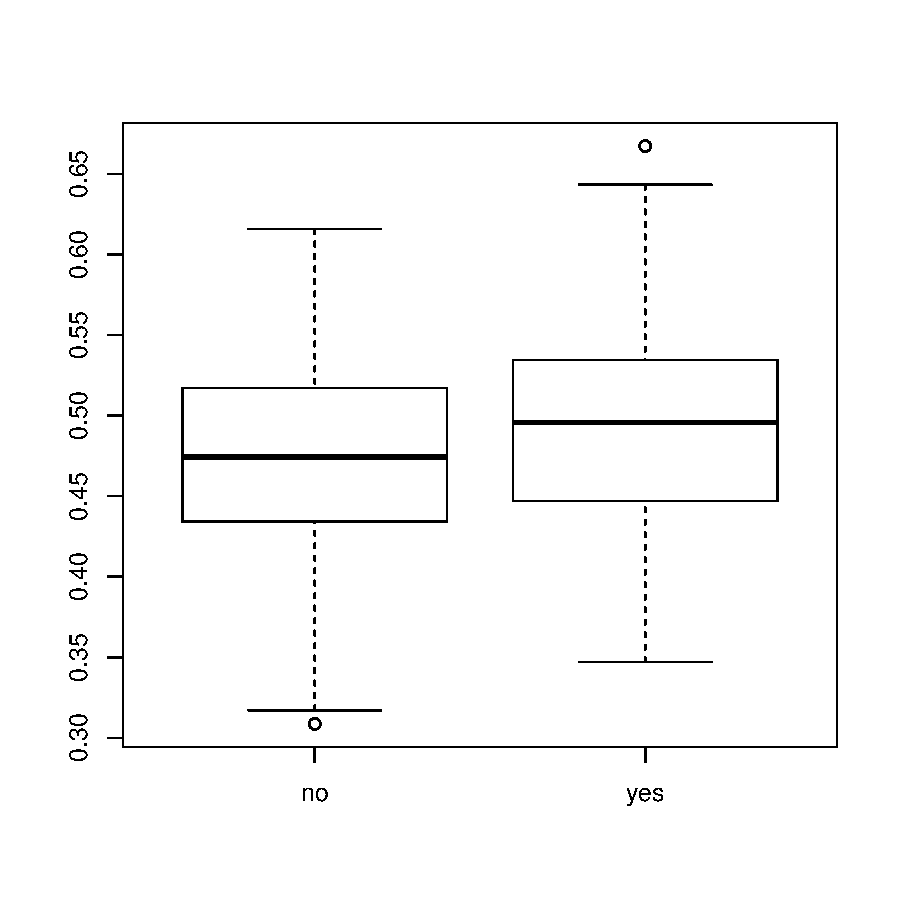
\includegraphics{analysis-035}

\begin{Schunk}
\begin{Sinput}
> wilcox.test(dur_word ~ asp, data = bi)
\end{Sinput}
\begin{Soutput}
	Wilcoxon rank sum test with continuity correction

data:  dur_word by asp
W = 17288, p-value = 0.00254
alternative hypothesis: true location shift is not equal to 0
\end{Soutput}
\end{Schunk}

According to a Wilcoxon-test, the duration of bisyllabic words is affected by the presence vs. absence of preaspiration.


\begin{Schunk}
\begin{Sinput}
> boxplot(dur_word ~ asp, data = results)
> shapiro.test(results$dur_word[bi$asp == "yes"])
\end{Sinput}
\begin{Soutput}
	Shapiro-Wilk normality test

data:  results$dur_word[bi$asp == "yes"]
W = 0.99087, p-value = 0.02167
\end{Soutput}
\begin{Sinput}
> shapiro.test(results$dur_word[bi$asp == "no"])
\end{Sinput}
\begin{Soutput}
	Shapiro-Wilk normality test

data:  results$dur_word[bi$asp == "no"]
W = 0.9956, p-value = 0.243
\end{Soutput}
\end{Schunk}
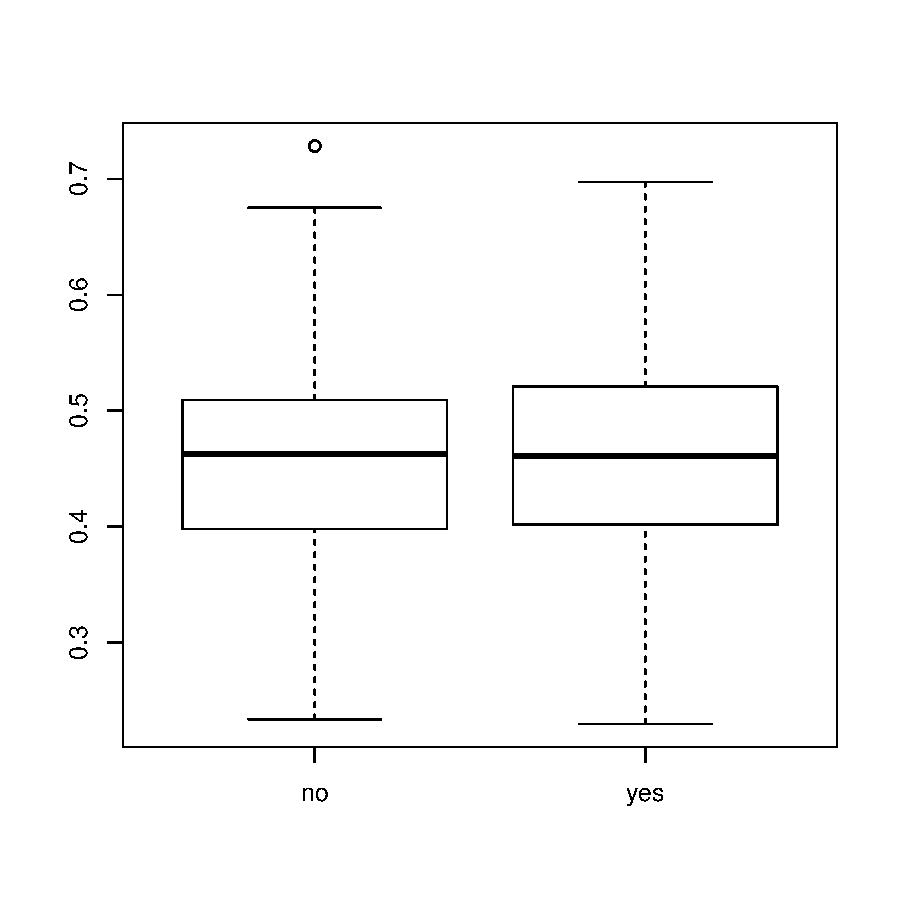
\includegraphics{analysis-037}

\begin{Schunk}
\begin{Sinput}
> wilcox.test(dur_word ~ asp, data = results)
\end{Sinput}
\begin{Soutput}
	Wilcoxon rank sum test with continuity correction

data:  dur_word by asp
W = 79777, p-value = 0.2782
alternative hypothesis: true location shift is not equal to 0
\end{Soutput}
\end{Schunk}

\end{document}
